\chapter{HIỆN TẠI VÀ TƯƠNG LAI: YOLO26 (2026)}

\textbf{Tác giả:} Ultralytics \hfill \textit{Không có paper chính thức} \cite{yolo26}\\
\textit{Phiên bản mới nhất tính đến thời điểm viết báo cáo --- ``trùm cuối'' của dòng Ultralytics.}

\section{Tại sao gọi ``YOLO26'' thay vì ``YOLOv13''?}
Từ YOLO11 (2024), Ultralytics bỏ tiền tố ``v''. Đến phiên bản tiếp theo, thay vì ``YOLO12'' (trùng YOLOv12 của Tian et al. \cite{yolov12}), Ultralytics dùng \textbf{quy tắc đặt tên theo năm}: YOLO\textbf{26} = năm 20\textbf{26}.

\section{Bỏ DFL --- Thay đổi triết lý lớn nhất}

DFL (Distribution Focal Loss, v8--v12) dự đoán phân phối 16 bins/coordinate $\rightarrow$ tốt accuracy nhưng \textbf{phức tạp cho edge deployment}. YOLO26 bỏ DFL, quay về dự đoán trực tiếp, bù bằng 3 training techniques mới.

\subsection{Phân tích kỹ thuật: Tại sao bỏ DFL?}

\textbf{Chi phí Memory Access Cost (MAC) của DFL:}

Với DFL 16 bins, mỗi anchor cần dự đoán $4 \times 16 = 64$ giá trị cho box regression (thay vì 4 giá trị trực tiếp). Trên toàn feature pyramid 3 scales ($80 \times 80 + 40 \times 40 + 20 \times 20 = 8400$ anchors):

\begin{equation}
\text{MAC}_{DFL} = 8400 \times 64 \times 4\text{B} = 2.15\text{MB/frame}
\end{equation}
\begin{equation}
\text{MAC}_{Direct} = 8400 \times 4 \times 4\text{B} = 0.13\text{MB/frame}
\end{equation}

Bỏ DFL giảm \textbf{16$\times$ bandwidth} cho box regression head. Trên NPU rẻ tiền (Jetson Nano, RK3588) có bus hẹp, đây là bottleneck nghiêm trọng. So sánh:

\begin{table}[H]\centering
\caption{So sánh overhead: DFL vs Direct vs Attention trên NPU}
\begin{tabular}{lccc}\toprule
\textbf{Component} & \textbf{MAC/frame} & \textbf{INT8 friendly?} & \textbf{NPU support}\\\midrule
DFL 16-bin (v8--v12) & 2.15 MB & Trung bình & Cần custom op \\
Direct regression (YOLO26) & 0.13 MB & \textbf{Tốt nhất} & \textbf{Native} \\
Area Attention (v12) & $\sim$5 MB & Kém (cần FP16) & Hạn chế \\\bottomrule
\end{tabular}
\end{table}

\textit{Kết luận:} YOLO26 ``Edge-First'' không chỉ nhanh hơn trên CPU, mà thực sự tối ưu \textbf{bandwidth và compatibility} trên NPU --- thân thiện với INT8 quantization và các chip AI giá rẻ. YOLOv12 (Attention-centric) tuy mạnh nhưng \textbf{cần FlashAttention trên GPU}, không chạy tốt trên NPU.

%% ========== MuSGD ==========
\section{MuSGD (Muon-enhanced SGD)}

\textbf{Vấn đề:} SGD truyền thống cập nhật: $\theta_{t+1} = \theta_t - \eta \nabla_\theta \mathcal{L}$. Hội tụ chậm khi loss landscape phức tạp.

\textbf{Giải pháp --- Muon momentum:} Muon (phát triển cho LLM) sử dụng momentum trên nhóm trực giao (orthogonal group). Công thức cập nhật:

\begin{equation}
m_{t+1} = \beta \cdot m_t + (1-\beta) \cdot \nabla_\theta \mathcal{L}_t
\end{equation}
\begin{equation}
\hat{m}_{t+1} = \text{NewtonSchulz}(m_{t+1}) \approx U \Sigma^{-1/2} V^T \quad \text{(xấp xỉ SVD)}
\end{equation}
\begin{equation}
\theta_{t+1} = \theta_t - \eta \cdot \hat{m}_{t+1}
\end{equation}

Trong đó $\text{NewtonSchulz}$ là phép lặp Newton-Schulz xấp xỉ phân rã SVD trong 5 bước (thay vì $O(n^3)$ của SVD đầy đủ). Hiệu ứng: gradient được \textbf{chuẩn hóa trên manifold trọng số}, tránh kẹt ở local minima \cite{yolo26}.

\begin{analogybox}
\textbf{Leo núi trong sương mù:} SGD giống bạn chỉ cảm nhận \textbf{độ dốc ngay dưới chân} rồi bước xuống --- dễ kẹt ở thung lũng nhỏ. MuSGD giống có thêm \textbf{la bàn chiến lược} (Muon momentum) nhìn được xu hướng địa hình rộng hơn --- khi gặp thung lũng nhỏ, la bàn chỉ bạn bước qua vì phía sau còn thung lũng sâu hơn.
\end{analogybox}

\textbf{Hiệu quả:} Thay thế AdamW (v8--v12) mà accuracy tương đương hoặc cao hơn, ít memory hơn.

%% ========== STAL ==========
\section{STAL (Small-Target-Aware Label Assignment)}

\textbf{Vấn đề:} TAL \cite{ppyoloe} dùng alignment metric $t = s^\alpha \cdot u^\beta$ (cls score $s$, IoU $u$). Vật nhỏ có IoU tự nhiên thấp $\rightarrow$ ít positive samples.

\textbf{Giải pháp --- Dynamic threshold:}

\begin{equation}
\tau(A_{gt}) = \tau_{base} \cdot \left(\frac{A_{max}}{A_{gt}}\right)^{\gamma}, \quad \gamma \in [0.3, 0.5]
\end{equation}

Trong đó $A_{gt}$ là diện tích ground truth, $A_{max}$ là diện tích GT lớn nhất trong batch, $\gamma$ kiểm soát mức nới lỏng. Khi $A_{gt}$ nhỏ $\rightarrow$ $\tau$ giảm $\rightarrow$ nhiều predictions đạt ngưỡng positive hơn \cite{yolo26}.

\begin{analogybox}
\textbf{Thầy giáo ưu tiên học sinh yếu:} Học sinh giỏi (vật lớn) luôn được khen --- đã có motivation. Học sinh yếu (vật nhỏ) ít được chú ý. STAL hạ tiêu chuẩn khen thưởng cho nhóm yếu (nới $\tau$), để các em nhận nhiều feedback tích cực hơn $\rightarrow$ dần cải thiện.
\end{analogybox}

\textbf{Hiệu quả:} Đặc biệt tốt cho \textbf{drone, camera giám sát tầm xa}, nơi vật thể thường rất nhỏ.

%% ========== ProgLoss ==========
\section{ProgLoss (Progressive Loss Balancing)}

\textbf{Vấn đề:} YOLO loss: $\mathcal{L} = \lambda_{cls} \mathcal{L}_{cls} + \lambda_{box} \mathcal{L}_{box} + \lambda_{obj} \mathcal{L}_{obj}$. Truyền thống dùng $\lambda$ cố định.

\textbf{Giải pháp --- Adaptive scheduling:}

\begin{equation}
\lambda_{cls}(t) = \lambda_{cls}^{max} - (\lambda_{cls}^{max} - \lambda_{cls}^{min}) \cdot \frac{t}{T}
\end{equation}
\begin{equation}
\lambda_{box}(t) = \lambda_{box}^{min} + (\lambda_{box}^{max} - \lambda_{box}^{min}) \cdot \frac{t}{T}
\end{equation}

Với $t$ = epoch hiện tại, $T$ = tổng epochs. Giai đoạn đầu ($t \ll T$): $\lambda_{cls}$ cao, $\lambda_{box}$ thấp $\rightarrow$ model học nhận diện trước. Giai đoạn sau ($t \to T$): $\lambda_{box}$ tăng $\rightarrow$ tinh chỉnh vị trí.

\begin{analogybox}
\textbf{Học lái xe:} Tuần đầu: giáo viên dạy \textbf{nhận biết biển báo} (cls). Tuần sau: chuyển sang \textbf{căn đường, đỗ xe chính xác} (reg). Nếu dạy cả hai cùng tỷ lệ từ đầu ($\lambda$ cố định), bạn sẽ quá tải.
\end{analogybox}

\textbf{Hiệu quả:} +0.3--0.5\% mAP so với fixed $\lambda$, đặc biệt khi bỏ DFL.

%% ========== Kết quả ==========
\section{Kết quả}
\begin{table}[H]\centering
\caption{YOLO26 so với YOLO11 và YOLOv12 (COCO val, input 640)}
\begin{tabular}{lccccl}\toprule
\textbf{Model} & \textbf{Params} & \textbf{mAP@50:95} & \textbf{CPU (ms)} & \textbf{GPU (ms)} & \textbf{Ghi chú}\\\midrule
YOLO11-N & 2.6M & 39.5\% & 76 & 1.6 & Baseline \\
\textbf{YOLO26-N} & \textbf{$\sim$2.5M} & \textbf{$\sim$40.5\%} & \textbf{43} & \textbf{1.4} & +1.0\%, CPU nhanh 43\% \\
YOLO11-S & 9.4M & 47.0\% & --- & 2.5 & --- \\
\textbf{YOLO26-S} & \textbf{$\sim$9M} & \textbf{$\sim$47.5\%} & --- & \textbf{2.1} & +0.5\% \\
YOLOv12-X & 59.1M & 55.2\% & --- & 12.1 & Cần FlashAttention \\
\textbf{YOLO26-X} & \textbf{$\sim$60M} & \textbf{$\sim$57.2\%} & --- & \textbf{9.8} & \textbf{SOTA, NPU-friendly} \\\bottomrule
\end{tabular}
\end{table}

\textit{Ghi chú: Số liệu ước tính từ benchmark cộng đồng, chưa có paper chính thức. CPU = ONNX Runtime trên i7-12700. GPU = TensorRT FP16 trên T4 \cite{yolo26}.}

YOLO26-X ($\sim$57.2\%) \textbf{vượt kỷ lục mAP} của v7-E6E (56.8\% \cite{yolov7}) --- lần đầu sau 4 năm.

\section{Tổng kết triết lý YOLO26}
YOLO26 đại diện cho xu hướng \textbf{``less is more''}: bỏ component phức tạp (DFL), thay bằng training techniques (MuSGD, STAL, ProgLoss). Kết quả: model nhẹ hơn, nhanh hơn trên CPU/NPU, accuracy vẫn SOTA --- \textbf{đúng nghĩa Edge-First Design}.

\begin{figure}[H]
\centering
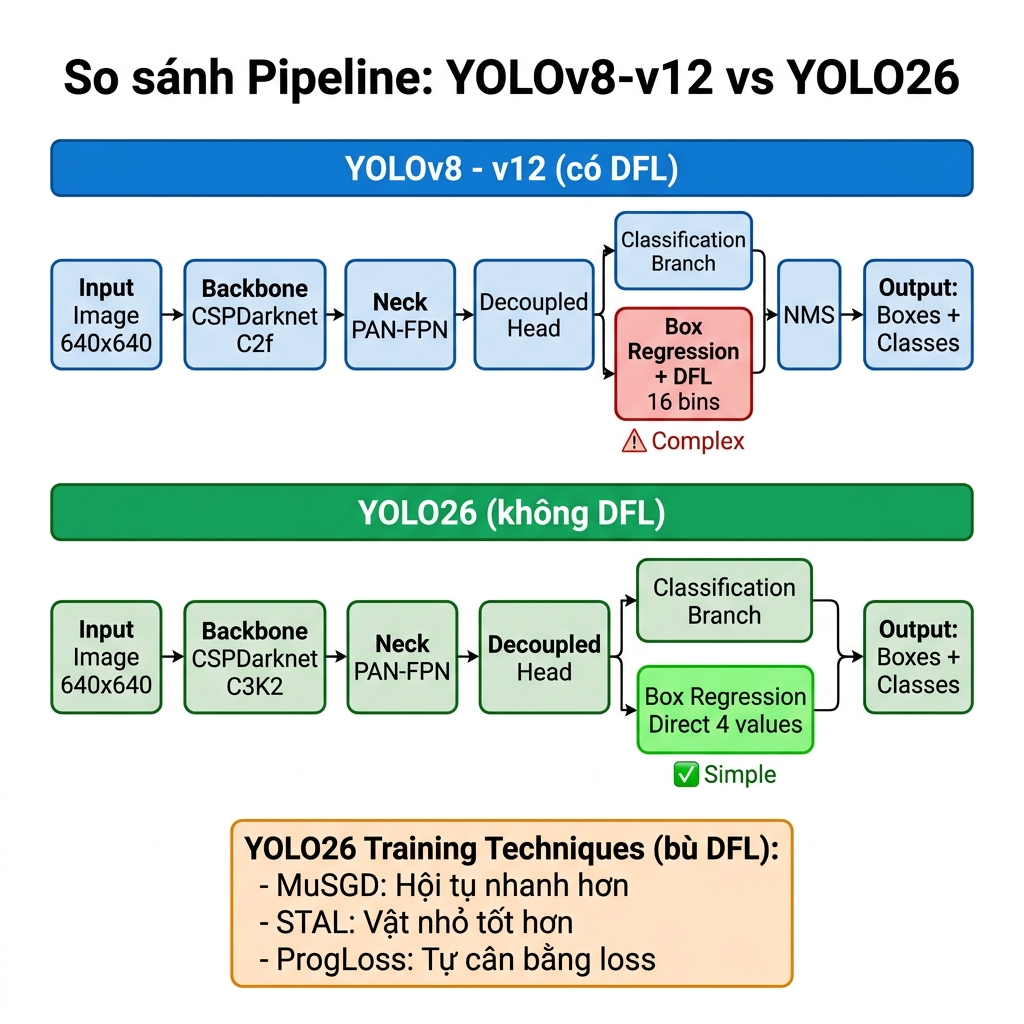
\includegraphics[width=\textwidth]{yolo26_pipeline.png}
\caption{So sánh pipeline: YOLOv8--v12 (có DFL) vs YOLO26 (không DFL). YOLO26 bù bằng 3 training techniques: MuSGD, STAL, ProgLoss.}
\end{figure}
